% Chapter 5

\chapter{Chapter 5: Model Fitting and Model Simulation} % Main chapter title

\label{Chapter 5} % For referencing the chapter elsewhere, use \ref{Chapter5} 

%----------------------------------------------------------------------------------------
\section{Possible Models}
\label{sec:Possible Models}
\paragraph{}
We have reviewed several classic models in Chapter \ref{Chapter 2}. But what kind of model is possible in this specific task? We will firstly give some intuitions, detailly describe their algorithms and make hypotheses in this section, then do model fitting in Section \ref{sec:Model Fitting}. Finally, we will see whether the best model could capture several features in participants' data in Section \ref{sec:Model Simulation} with Model Simulation. 

\subsection{Model-Free Models}
\paragraph{}
Model-Free algorithms in this task need to maintain three different Q value tables for three tasks because the goal state has three possibilities: \emph{A}, \emph{B} and \emph{C}. Therefore, we should create 3 Q value tables for two kinds of classic Model-Free algorithm, SARSA and Q-learning. The difference between SARSA and Q-learning is that when calculating reward prediction error (RPE), SARSA uses the true action chosen by participants in the next timestep, while Q-learning uses the action with maximum Q value on the next state. We rewrite the update rule for SARSA and Q-learning here in Equation \ref{eqn:SARSA} and \ref{eqn:Q-Learning}, in which $\alpha$ is learning rate, $\gamma$ is temporal discounting factor. 

\begin{equation}
\begin{aligned}
&\delta_{RPE}=r(s^{\prime})+\gamma Q_{SARSA}(s^{\prime}, a^{\prime})-Q_{SARSA}(s,a) \\
&Q_{SARSA}(s,a)=Q_{SARSA}(s,a)+\alpha \delta_{RPE} \\
\end{aligned}
\label{eqn:SARSA}
\end{equation}

\begin{equation}
\begin{aligned}
&\delta_{RPE}=r(s^{\prime})+\gamma \max_{a^{\prime} \in a(s)}{Q_{Q}(s^{\prime}, a^{\prime})}- Q_{Q}(s,a) \\
&Q_Q(s,a)=Q_Q(s,a)+\alpha \delta_{RPE} \\
\end{aligned}
\label{eqn:Q-Learning}
\end{equation}

\paragraph{}
What's more, considering the difficulty of this task, we add forget rate into the model as Equation \ref{eqn:MF forget} in which $f$ represents forget rate ranging from 0 to 0.05. Note that the reason why the maximum $f$ is only 0.01 is that we assume forget takes place at every timestep in every trial. If it takes the participants averagely 10 steps to get to the end state, then after 10 trials the participants will almost totally forget the Q value of that state ($(1-0.05)^{10 \times 45} \approx 0.005$). 

\begin{equation}
\begin{aligned}
&Q(s,a)=Q(s,a) \times (1 - f) \\
\end{aligned}
\label{eqn:MF forget}
\end{equation}

\paragraph{}
The decision probability is determined by softmax's transformation of Q value according to Equation \ref{eqn:softmax}, in which $\tau$ is inverse temperature determining how much the participants will prefer the action with higher Q value. If $\tau = 0$, each action will receive a same probability to be chosen. If $\tau = \infty$, participants will definitely choose the action with highest Q value. 

\begin{equation}
\begin{aligned}
P(a)=\frac{e^{\tau Q(s,a)}}{\sum_a{e^{\tau Q(s,a)}}}
\end{aligned}
\label{eqn:softmax}
\end{equation} 


\subsection{Model-Based Models}
\paragraph{}
Unlike Model-Free algorithm, Model-Based algorithm only maintain one set of transition matrix. In this task, we assume that participants do not need to learn reward function, since the reward function is rather simple: rewards in the end state (depend on how many steps it takes) and 0 elsewhere. The transition learning method we apply is similar to \cite{glascher2010states} with a state prediction error (SPE). The update rule is shown in Equation \ref{eqn:Transition Update}, in which $\eta$ is learning rate, $s^{\prime} is the observed new state$. It is obvious that after every update of $T$, $\sum_{s^{\prime \prime}}T(s,a)=1$, keeping the distribution normalized. 

\begin{equation}
\begin{aligned}
&\delta_{SPE}=1-T(s,a,s^{\prime}) \\
&T(s,a,s^{\prime})=T(s,a,s^{\prime})+\eta \delta_{SPE} \\
&T(s,a,s^{\prime \prime})=T(s,a,s^{\prime \prime})\times(1-\eta) \quad \forall s^{\prime \prime} \neq s^{\prime}
\end{aligned}
\label{eqn:Transition Update}
\end{equation}

\paragraph{}
In the Model-Based methods, participants need to do extra calculation to gain value estimation. \citet{glascher2010states} use a dynamic programming (see Equation \ref{eqn:Backforward Q}) to calculate the Q value using transition matrix and reward information. We apply the same method in our pure Model-Based methods, but it is worth noting that dynamic programming is viable in their experiment because it is only a simple two stage decision with now states shared between stages. However, this task of ours is much complicated and the same state may be visited more than once in a trial, which makes dynamic programming much harder to converge. Actually, in \citeauthor{glascher2010states}'s experiment it is guaranteed to be convergent with two iterations. But in our experiment settings, it seems there is no clear guarantee of convergence. Considering the computation limit of human brain, we still iterate the dynamic programming equation two times, but reader should be aware of the limit of this method. This method is actually a simplified value iteration algorithm in Computer Science \cite{sutton1998introduction}. There does exist other algorithms such as policy iteration, but they suffer from the same problem of computation complexity. Therefore, we only consider value iteration in pure Model-Based method in this thesis. 

\begin{equation}
\begin{aligned}
Q(s,a)=\sum_{s^{\prime}}T(s,a,s^{\prime})\times(r(s^{\prime})+\arg \max_{a^{\prime}}Q(s^{\prime},a^{\prime}) )
\end{aligned}
\label{eqn:Backforward Q}
\end{equation}

\paragraph{}
Similar to Model-Free method, we add forget rate in Model-Based Models as well. The difference between Model-Free forget and Model-Based forget is that Model-Free forget is toward 0 while Model-Based forget in our experiment is toward $\frac{1}{6}$, since the uniform distribution of transition will result in $\frac{1}{6}$. The forget process is given by Equation \ref{eqn:MB forget}, in which $f$ is the forget rate. 

\begin{equation}
\begin{aligned}
&T(s,a,s^{\prime})=(\frac{1}{6} - T(s,a,s^{\prime})) \times f + T(s,a,s^{\prime}) \\
\end{aligned}
\label{eqn:MB forget}
\end{equation}


\paragraph{}
After the Model-Based value has been calculated, action selection follows the same softmax transformation as Equation \ref{eqn:softmax}. 

\subsection{Hybrid Model}
\label{sec:Hybrid Model}
\paragraph{}
A Hybrid learner combines state-action value estimates from both Model-Free and Model-Based. This model assumes that human brain has two kinds of learning mechanism, model-free and model-based, and when making decisions they produce two value estimation simultaneously. Following \citet{bucci1998removal}, we characterize the weight with an exponential function (see Equation \ref{eqn:Hybrid Weight}). % TODO Hybrid MF use Q or SARSA
\begin{equation}
\begin{aligned}
w_t=I\times e^{-kt}
\end{aligned}
\label{eqn:Hybrid Weight}
\end{equation}

\paragraph{}
Q value calculation for Hybrid model is shown in Equation \ref{eqn:Hybrid value}. 
\begin{equation}
\begin{aligned}
Q_{HYB}(s,a)=w_t\times Q_{MB}(s,a)+(1-w_t)\times Q_{MF}(s,a)
\end{aligned}
\label{eqn:Hybrid value}
\end{equation}

\paragraph{}
After the hybrid value has been calculated, action selection follows the same softmax transformation as Equation \ref{eqn:softmax}. 


\subsection{Model-Based Help Model-Free Model}
\label{sec:Model-Based Help Model-Free Model}
\paragraph{}
Model-Free models suffer from incorrect inference. For example, the participant is now at \emph{E} and his  goal is \emph{B}. At this time the participant choose the action whose primary consequence is \emph{D} but with $0.2$ probability it is transited to \emph{B}, and he win the reward. In this situation, Model-Free models will credit the action whose primary consequence is \emph{D}, which is obviously unwise. However, since Model-Based methods is aware of which action's primary consequence is the reward state, it should be able to \enquote{help} Model-Free methods to fix this kind of wrong credit. Thus, the Model-Based Help Model-Free Model, or in short MBHMF Model, does Model-Free and Model-Based learning simultaneously as Hybrid model, but it only relies on Model-Free prediction to do decision making. On the other hand, when Model-Free is updating its value, it will check whether the action chosen by participant is the most likely transit-to-the-new-state one. If it is not, and another action has more than $0.7$ probability to transit to this new state, it will fix the mistake. The mathematical formulation of mistake fixing is shown in Equation \ref{eqn:MB help MF Q-Learning}. 

\begin{equation}
\begin{aligned}
&\delta_{RPE}=r(s^{\prime})+\gamma \max_{a^{\prime} \in a(s)}{Q_{Q}(s^{\prime}, a^{\prime})}- Q_{Q}(s,a^{\prime \prime}) \\
&Q(s,a^{\prime \prime})=Q(s,a^{\prime \prime})+\alpha \delta_{RPE} \\
&T(s,a^{\prime \prime},s^{\prime}) > T(s,a^{\prime \prime \prime},s^{\prime}) \quad \forall a^{\prime \prime \prime}\neq a^{\prime \prime} \\
&T(s,a^{\prime \prime},s^{\prime}) > 0.7 \\
\end{aligned}
\label{eqn:MB help MF Q-Learning}
\end{equation}

\paragraph{}
Action selection of MBHMF model follows the same softmax transformation as Equation \ref{eqn:softmax}. 

\subsection{Model-Free Help Model-Based Model}
\label{sec:Model-Free Help Model-Based Model}
\paragraph{}
Model-Based could fix mistakes in Model-Free learning. Can Model-Free help Model-Based method as well? The answer is yes. 
\paragraph{}
First of all, Model-Free could help reducing the extreme computational burden when calculating value estimation. In fact, Model-Free value estimation could help Model-Based Model doing successor matrix calculation, which could easily be turned to value by right dot product reward vector. This method is named Model-Free Help Model-Based (MFHMB) model. Its value estimation is totally determined by Model-Based calculation. 
\paragraph{}
Specifically, the successor matrix $S$ is given by Equation \ref{eqn:Successor Matrix}. Successor matrix represents from current state, taking action a, how much probability I will be in every state. $I_t$ in the equation means the probability of each state after $t$ step transitions. The first equation in \ref{eqn:Successor Matrix} shows that in one step, the successor matrix is just equal to the transition matrix on current state and specific action. The second equation represents that after first transition, the action chosen by algorithm will be the action that has maximum Model-Free Q value, resulting in a greedy policy. After the action have been chosen, the second equation could calculate the probability of each state's probability after two steps transition from current state. Then the third, fourth transition can be calculated in the same manner. Successor matrix $S(a,s)$ is just a sum of all $I_t$ with temporal discounting. As the basic Model-Based method, we could just calculate two steps from current state to match the computational ability of human brain. Previous Model-Based value estimation's computation complexity is $\mathcal{O}(S^2AI)$, in which $S$ is the number of all states, $A$ is the number of all actions and $I$ is iteration time. However, successor matrix calculation's computation complexity is decrease to $\mathcal{O}(SAI)$. 

\begin{equation}
\begin{aligned}
&I_1(a,s^{\prime}) = T(s,a,s^{\prime}) &\text{s is the current state} \\
&I_t(a,s^{\prime}) = I_{t-1}(a,s)\times T(s,a^{\prime},s^{\prime}) \quad a^{\prime}=\arg \max_{a}{Q_{MF}(s,a)} \quad & t=2,3,... \\
&S(a,s) = \sum_{t=1}^{\infty}{\gamma^{t-1}I_t} &\text{s is sucessor state} \\
\end{aligned}
\label{eqn:Successor Matrix}
\end{equation}

\paragraph{}
Successor matrix could easily be transformed to value by Equation \ref{eqn:Sucessor Matrix Value}, in which $R$ is the reward function. Note that $s$ could only be the current state since we do not calculate successor matrix from other states. 

\begin{equation}
\begin{aligned}
Q(s,a) = \sum_{s^{\prime}}S(a,s^{\prime})R(s^{\prime}) 
\end{aligned}
\label{eqn:Sucessor Matrix Value}
\end{equation}


\paragraph{}
Action selection of MFHMB model follows the same softmax transformation as Equation \ref{eqn:softmax}. 

\subsection{Conclusion of Models}
\label{sec:Conclusion of Models}
\paragraph{}
In this section we introduced five models, including MF model, MB model, Hybrid model, MBHMF model, MFHMB model. They are summarized in Table \ref{table:Possible Models} and their parameters are summarized in Table \ref{table:Model Parameters}. Readers could easily observe that MF model and MB model is two base models while other two models are built upon them. In the meantime, the idea of Hybrid, MBHMF, MFHMB are not mutual-exclusive, which means they could exist as a whole. Due to the time limit, we could not examine models combining two or three ideas but leave this as a feature work direction. 

\begin{table}
\caption{Possible Models}
\label{table:Possible Models}
\centering
\begin{tabular}{l l c}
\toprule
\tabhead{Model Name} & \tabhead{Abbreviation} & \tabhead{Parameters} \\
\midrule
Model-Free & MF & $\alpha$, $\tau$, $\gamma$, $f_{MF}$ \\
Model-Based & MB & $\eta$, $\tau$, $\gamma$, $f_{MB}$ \\
Hybrid & Hybrid & $\alpha$, $\eta$,  $\tau$, $\gamma$, $f_{MF}$, $f_{MB}$, $I$, $k$ \\
Model-Based Help Model-Free & MBHMF & $\alpha$, $\eta$, $\tau$, $\gamma$, $f_{MF}$, $f_{MB}$ \\
Model-Free Help Model-Based & MFHMB & $\alpha$, $\eta$, $\tau$, $\gamma$, $f_{MF}$, $f_{MB}$ \\
\bottomrule\\
\end{tabular}
\end{table}

\begin{table}
\caption{Model Parameters}
\label{table:Model Parameters}
\centering
\begin{tabular}{c c c}
\toprule
\tabhead{Parameter Name} & \tabhead{Meaning} & \tabhead{Bound} \\
\midrule
$\alpha$ & learning rate of MF & [0, 1] \\
$\eta$ & learning rate of MB & [0, 1] \\
$\tau$ & inverse temperature in softmax & [0, $\infty$) \\
$\gamma$ & temporal discounting rate & [0, 1] \\
$f_{MF}$ & forget rate of MF & [0, 0.05] \\
$f_{MB}$ & forget rate fo MB & [0, 0.05] \\
$I$ & hybrid exponential function parameter & [0, 1] \\
$k$ & hybrid exponential function parameter & [0, 0.1] \\
\bottomrule\\
\end{tabular}
\end{table}

\paragraph{}
It is also worth mentioning that MB and MF could also assist or interfere with each other in many other ways. We have tried several other possibilities, such as MF limits MB learning (MB only learns when it is valuable). Since it has been plenty of evidence that MB and MF co-exist in our decision system, readers should be aware that there could exist pretty much possibilities that MB and MF cooperate or compete with each other we can't cover in this thesis. 


%----------------------------------------------------------------------------------------


%----------------------------------------------------------------------------------------
\section{Model Fitting}
\label{sec:Model Fitting}
\paragraph{}
All the data fitting procedures were conducted on the individual level using maximum likelihood estimates. We use a function \code{optimize.minimize} in SciPy(\cite{Scipy}) to search for the parameters that minimized minus log likelihood. To verify that we had found the global minimum, we repeated the search process using 12 different starting points.
\paragraph{}
We used Akaike information criterion with a correction for sample sizes (AICc) to do model comparison (\cite{akaike1974new}; \cite{bucci1998removal}). 
\paragraph{}
For each participant, we gained 5 AICc for 5 models. We then calculate the least AICc model for each participant. Firstly we compare Model-Free's 2 kinds of algorithms: SARSA and Q-learning. There are 31/36 participants that Q-learning has smaller AICc, indicating that Q-learning is much more possible and SARSA. Therefore, we will use Q-learning to complete the model free part in the Hybrid model, MBHMF model and MFHMB model. 
\paragraph{}
Secondly we compare whether adding forget will result in a better fit. The data shows that 29/36 participants has smaller AICc when forget is considered. Moreover, we could see that in the block condition of Fig. \ref{fig:Optimal Percentage Participants}, \ref{fig:Inner Optimal Percentage Participants}, \ref{fig:Outer Optimal Percentage Participants}, \ref{fig:Last Optimal Percentage Participants}, the last block performance is worse than previous three one on the same task, suggesting there exists forget. Therefore, we could conclude that forget is a key part of model for our experiment and we will add forget into the Hybrid model, MBHMF model and MFHMB model. 
\paragraph{}
Finally we compare our five major models. The comparison method is the same as SARSA vs Q-learning, to check which one of 5 models has least AICc on individuals. The result is summarized in Table \ref{table:Model Comparison}. We could see that Model-Free has most best model results of 19, Hybrid 11 and MBHMF 5. It seems Q-learning Model-Free with forget model is the best among 5 models. We will carry out further analyses in the next section \enquote{Model Simulation} towards this result. 
\paragraph{}
There is another interesting result in the model comparison. In the 11 participants that fit best with Hybrid model, 10 participants are in block condition, which also means almost no one in randomized condition fit Hybrid model. We will discuss this result in Chapter \ref{Chapter 6} in detail. 

\begin{table}
\caption{Model Comparison}
\label{table:Model Comparison}
\centering
\begin{tabular}{l c c}
\toprule
\tabhead{Model Name} & \tabhead{Best count} \\
\midrule
Model-Free & 19 \\
Model-Based & 1 \\
Hybrid & 11 \\
Model-Based Help Model-Free & 5 \\
Model-Free Help Model-Based & 0 \\
\bottomrule\\
\end{tabular}
\end{table}

%----------------------------------------------------------------------------------------



%----------------------------------------------------------------------------------------
\section{Model Simulation}
\label{sec:Model Simulation}

\begin{figure}[ht]
\centering
\subfigure[Optimal Percentage]{
\begin{minipage}[t]{0.48\textwidth}
\centering
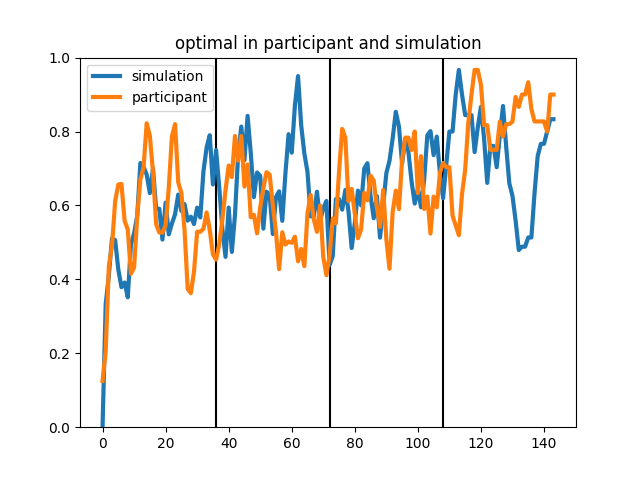
\includegraphics[width=\textwidth]{Figures/10_optimal}
\end{minipage}
}
\subfigure[Inner Optimal Percentage]{
\begin{minipage}[t]{0.48\textwidth}
\centering
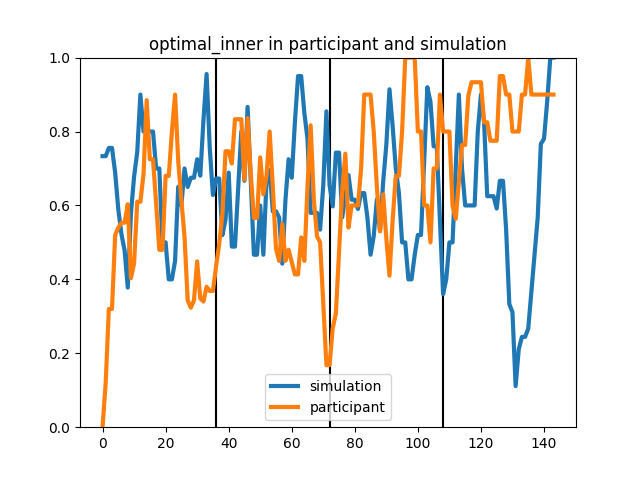
\includegraphics[width=\textwidth]{Figures/10_optimal_inner}
\end{minipage}
}
\\
\subfigure[Outer Optimal Percentage]{
\begin{minipage}[t]{0.48\textwidth}
\centering
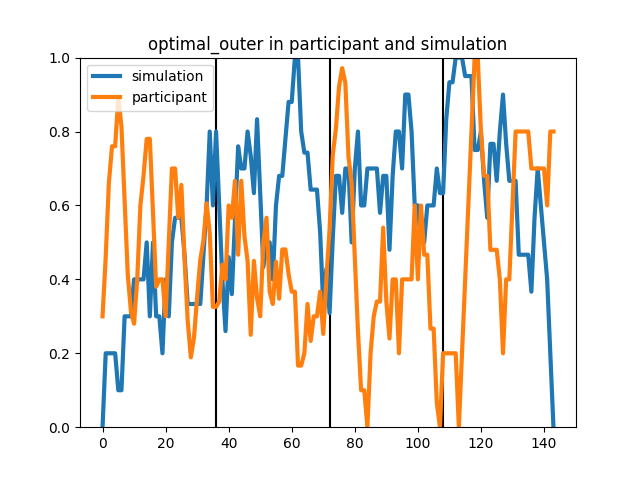
\includegraphics[width=\textwidth]{Figures/10_optimal_outer}
\end{minipage}
}
\subfigure[Last Optimal Percentage]{
\begin{minipage}[t]{0.48\textwidth}
\centering
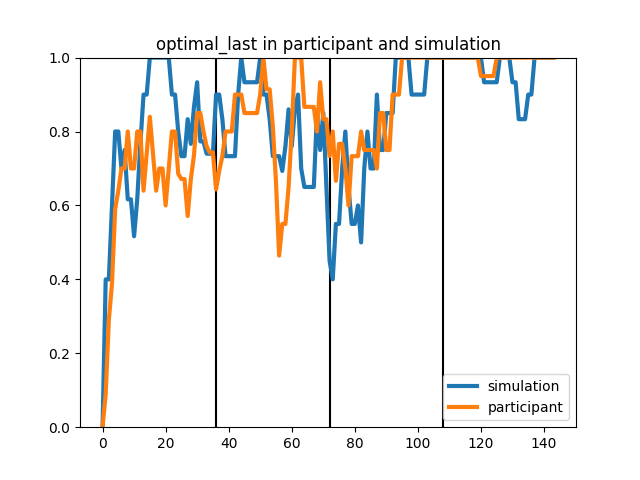
\includegraphics[width=\textwidth]{Figures/10_optimal_last}
\end{minipage}
}
\decoRule
\caption[Participant 10's data compared with Simulation]{Participant 10's data compared with Simulation}
\label{fig:Participant 10's data compared with Simulation}
\end{figure}

\paragraph{}
In this section, we want to see whether our best model, Q-learning with forget, could recreate patterns participants show in both randomized and block conditions. 
\paragraph{}
All data simulation uses the params from model fitting maximum likelihood method. Therefore, we create one simulation for each participant using their parameters under Model-Free Q-learning with forget model. It is worth noting that one simulation has strong stochasticity both due to action selection and environment transition randomness. The reason why we do not repeat the simulation several times to use the mean value is that participant's data is also only one observation. Mean values will be much smoother than participant's data because of averaging operation. 
% TODO add all simulation results in Appendix

\paragraph{}
Participant 10 and 24 is a typical example of the model simulation. Their data and simulated data are shown in Fig. \ref{fig:Participant 10's data compared with Simulation} and \ref{fig:Participant 24's data compared with Simulation}. All data patterns are reflected by simulation for participant 10 and 24. 


\begin{figure}[htb]
\centering
\subfigure[Optimal Percentage]{
\begin{minipage}[t]{0.48\textwidth}
\centering
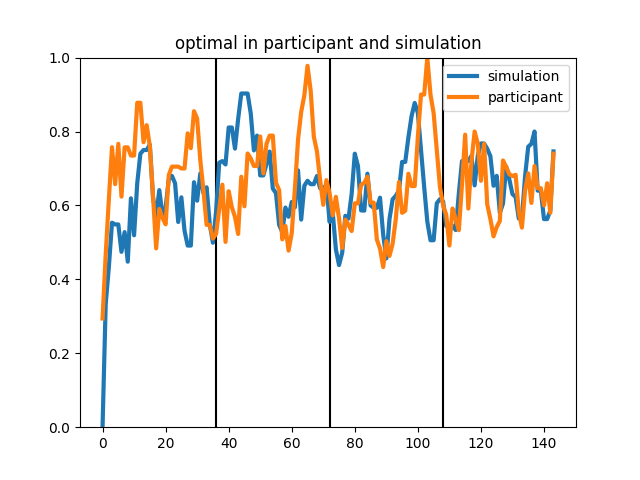
\includegraphics[width=\textwidth]{Figures/24_optimal}
\end{minipage}
}
\subfigure[Inner Optimal Percentage]{
\begin{minipage}[t]{0.48\textwidth}
\centering
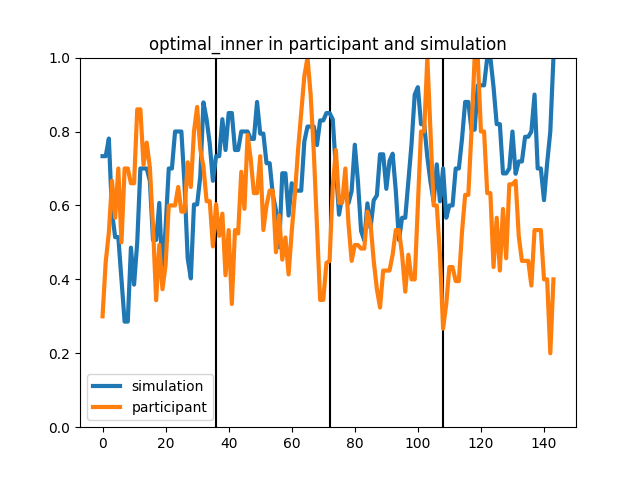
\includegraphics[width=\textwidth]{Figures/24_optimal_inner}
\end{minipage}
}
\\
\subfigure[Outer Optimal Percentage]{
\begin{minipage}[t]{0.48\textwidth}
\centering
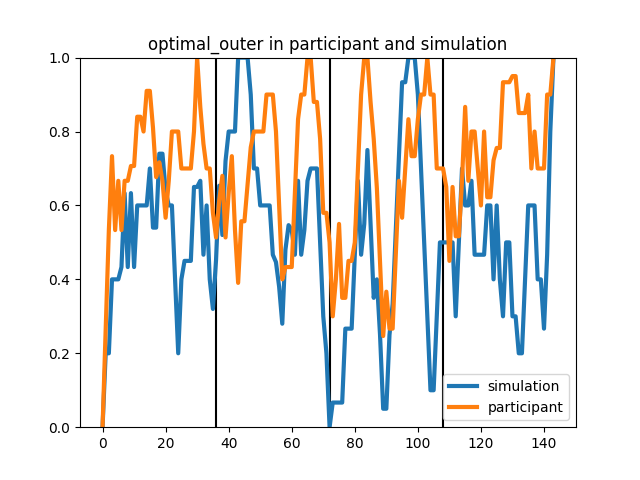
\includegraphics[width=\textwidth]{Figures/24_optimal_outer}
\end{minipage}
}
\subfigure[Last Optimal Percentage]{
\begin{minipage}[t]{0.48\textwidth}
\centering
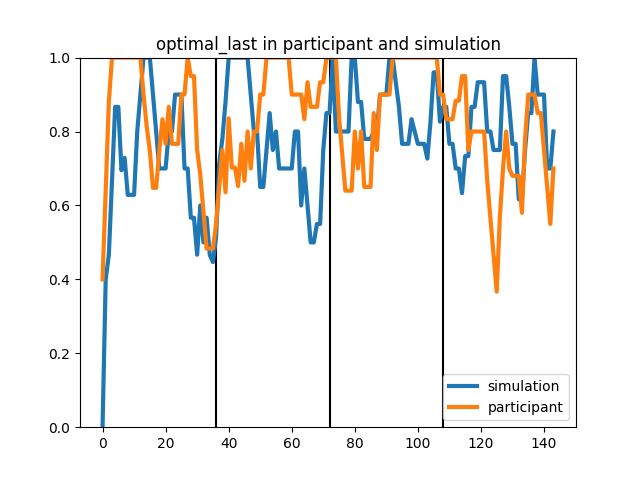
\includegraphics[width=\textwidth]{Figures/24_optimal_last}
\end{minipage}
}
\decoRule
\caption[Participant 24's data compared with Simulation]{Participant 24's data compared with Simulation}
\label{fig:Participant 24's data compared with Simulation}
\end{figure}


\paragraph{}
However, there still exist participants whose data pattern could not be captured by Model-Free model. For instance, participant 11 demonstrates a very bad performance in the beginning but soon climb to a very good performance (See Fig. \ref{fig:Participant 11's data compared with Simulation}). This seems not able to be captured by the Model-Free simulation. What's more, his best model is Hybrid model, which means the quickly increasing pattern may be a result of successfully Model-Based value estimation. 

\begin{figure}[htb]
\centering
\subfigure[Optimal Percentage]{
\begin{minipage}[t]{0.48\textwidth}
\centering
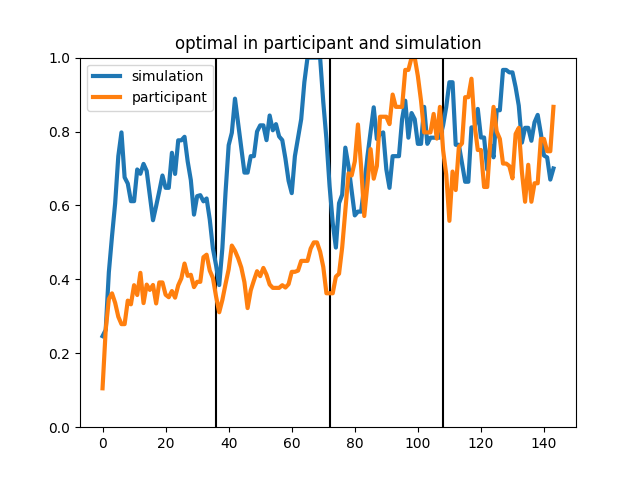
\includegraphics[width=\textwidth]{Figures/11_optimal}
\end{minipage}
}
\subfigure[Inner Optimal Percentage]{
\begin{minipage}[t]{0.48\textwidth}
\centering
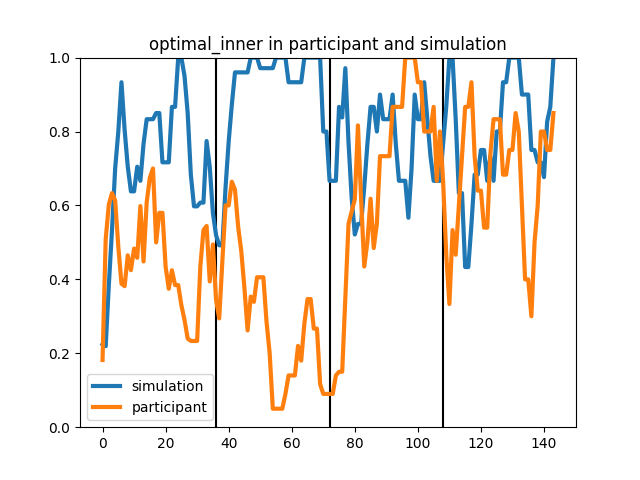
\includegraphics[width=\textwidth]{Figures/11_optimal_inner}
\end{minipage}
}
\\
\subfigure[Outer Optimal Percentage]{
\begin{minipage}[t]{0.48\textwidth}
\centering
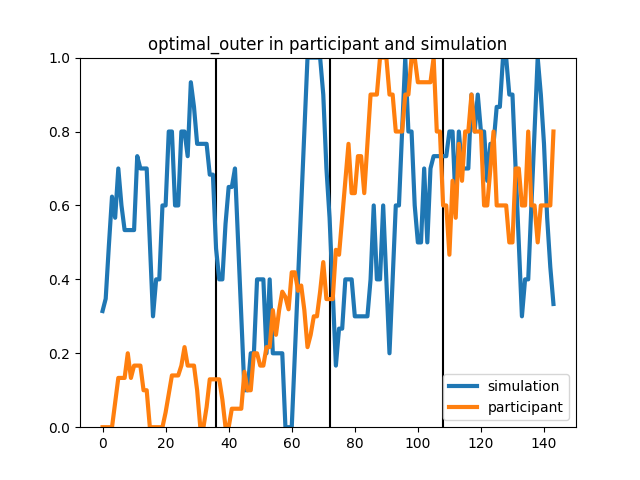
\includegraphics[width=\textwidth]{Figures/11_optimal_outer}
\end{minipage}
}
\subfigure[Last Optimal Percentage]{
\begin{minipage}[t]{0.48\textwidth}
\centering
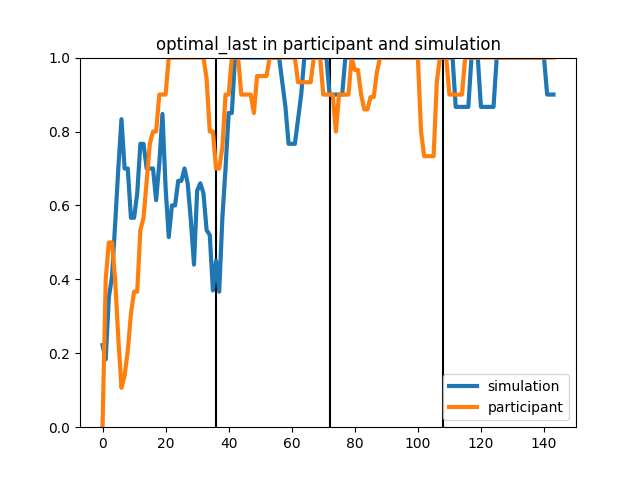
\includegraphics[width=\textwidth]{Figures/11_optimal_last}
\end{minipage}
}
\decoRule
\caption[Participant 11's data compared with Simulation]{Participant 11's data compared with Simulation}
\label{fig:Participant 11's data compared with Simulation}
\end{figure}

\paragraph{}
We also did model simulation in different parameters to see how will the data pattern change as the parameters change. Due to space limit, we put these graphs in the Appendix, while we describe some findings here. 
% add appendix ref

\paragraph{}
First of all, if the learning rate $\alpha$ or $\tau$ is close to 1, the performance will fluctuate a lot since it suffer from the stochasticity of environment transition. On the other hand, if the learning rate is close to 0, the learning will be much slower than the participants do. Therefore, a learning rate between 0.3 and 0.5 seems great in this task. 

\paragraph{}
Secondly, the softmax inverse temperature $\tau$ should never be too big or too small. If $\tau$ is close to 0, then the action selection is uniformly random regardless of value learned. If $\tau$ is bigger than 10, then the action selection will be too stable for the player, making him stuck in local optimum value. 

\paragraph{}
Finally, the forget rate. The average forget rate for participants is 0.0123, which means participants will totally forget in about 40 trials. This is reasonable because too small forget rate may result in sticking in local optimum since it can not forget the information, or transfer wrong knowledge to the following tasks. 

%----------------------------------------------------------------------------------------







